%%%%%%%%%%%%%%%%%%%%%%% file template.tex %%%%%%%%%%%%%%%%%%%%%%%%%
%
% This is a general template file for the LaTeX package SVJour3
% for Springer journals.          Springer Heidelberg 2010/09/16
%
% Copy it to a new file with a new name and use it as the basis
% for your article. Delete % signs as needed.
%
% This template includes a few options for different layouts and
% content for various journals. Please consult a previous issue of
% your journal as needed.
%
%%%%%%%%%%%%%%%%%%%%%%%%%%%%%%%%%%%%%%%%%%%%%%%%%%%%%%%%%%%%%%%%%%%
%
% First comes an example EPS file -- just ignore it and
% proceed on the \documentclass line
% your LaTeX will extract the file if required
\begin{filecontents*}{example.eps}
%!PS-Adobe-3.0 EPSF-3.0
%%BoundingBox: 19 19 221 221
%%CreationDate: Mon Sep 29 1997
%%Creator: programmed by hand (JK)
%%EndComments
gsave
newpath
  20 20 moveto
  20 220 lineto
  220 220 lineto
  220 20 lineto
closepath
2 setlinewidth
gsave
  .4 setgray fill
grestore
stroke
grestore
\end{filecontents*}
%
\RequirePackage{fix-cm}
%
%\documentclass{svjour3}                     % onecolumn (standard format)
%\documentclass[smallcondensed]{svjour3}     % onecolumn (ditto)
\documentclass[smallextended]{svjour3}       % onecolumn (second format)
%\documentclass[twocolumn]{svjour3}          % twocolumn
%
\smartqed  % flush right qed marks, e.g. at end of proof
%
\usepackage{graphicx}
\usepackage[colorlinks,linkcolor=red]{hyperref}
%
% \usepackage{mathptmx}      % use Times fonts if available on your TeX system
%
% insert here the call for the packages your document requires
%\usepackage{latexsym}
% etc.
%
% please place your own definitions here and don't use \def but
% \newcommand{}{}
%
% Insert the name of "your journal" with
% \journalname{myjournal}
%
\begin{document}

\title{Blind Image Quality Assessment with Grayscale-improved BIQI%\thanks{Grants or other notes
%about the article that should go on the front page should be
%placed here. General acknowledgments should be placed at the end of the article.}
}


%\titlerunning{Short form of title}        % if too long for running head

\author{Weipeng Wu         \and
        Chaoqun Hong     \thanks{Corresponding author: cqhong@xmut.edu.cn}\and
        Yong Xie \and
        Liang Chen
}

%\authorrunning{Short form of author list} % if too long for running head

\institute{Weipeng Wu\at
              School of Computer and Information Engineering, Xiamen University of Technology, Xiamen 361024, China. \\
              Tel.: 15359266643\\
              \email{weipengw0306@163.com}           %  \\
%             \emph{Present address:} of F. Author  %  if needed
\\
      \and
            Chaoqun Hong \at
            School of Computer and Information Engineering, Xiamen University of Technology, Xiamen 361024, China.\\   
\\	 \email{cqhong@xmut.edu.cn} 
        \and
           Yong Xie \at
            School of Computer and Information Engineering, Xiamen University of Technology, Xiamen 361024, China.\\
              \email{yongxie@xmut.edu.cn} 
         \\
                    \and
           Liang Chen \at
            School of Data and Computer Science, Sun Yat-Sen University, Guangzhou 510006, China.\\
              \email{Chenliang6@mail.sysu.edu.cn} 
    \\
}

\date{Revised: 3, Feb}
% The correct dates will be entered by the editor


\maketitle

\begin{abstract}
Image Quality Assessment (IQA) is a popular issue recently all over the world. Its function is to evaluate the levels of distortions in images with all kinds of distorted types. No-reference (NR) quality assessment methods do not need any reference image in evaluating the quality of the images. And these methods generally based on the statistical characters. On the other hand, most of IQA methods can not get positive results from images with multiple distorted types and levels. Recently, some problems above mentioned have been tackled by using Blind Image Quality Index (BIQI), but there still exists lots of intractable and urgent points that need new algorithm to solve, such as low sharpness, the high value of grayscale and so forth. In order to propose a new algorithm to tackle effectively these problems, we compare various factors that influence the results in IQA, and discuss some merits and demerits about the proposed algorithm. In this paper, the classification and proportions of distorted types will be classified and computed by using the proposed algorithm. The algorithm with No-Reference Structural Sharpness (NRSS) and grayscale can evaluate effectively the image quality. NRSS and grayscale are mainly embodied in extracting the structure features and obtaining the gradient information of the image. Lastly, lost of positive results about IQA are collected and they show that the proposed algorithm is closer to human visual judgement than other algorithm.
\keywords{Image Quality Assessment \and Blind Image Quality Index \and No-Reference Structural \and Sharpness \and Grayscale}

\end{abstract}

\section{Introduction}
\label{intro}
Recently, IQA has developed and the researchers have proposed numerous methods so that there are lots of effective solutions in IQA. Although the full-reference (FR) algorithms \cite{b1,b2,b3} and reduced-reference (RR) algorithms \cite{b4,b5,b6}have the high score in IQA, they are still limited in some practical applications. Another kind of algorithm is no-reference (NR) algorithm, and it is more useful for those researchers to conduct on experiments, because NR algorithms do not need to take a reference image and then this can assume images directly.

Nowadays, NR algorithms basically assess images with single distortion type during the process of assuming \cite{b7}. Besides, for an image with a certain kind of distortion type, most of NR algorithms can get the accurate results. On the contrary, if an image carries multiple types of distortion, the accuracy will be reduced greatly. However, in practical situation, the images usually have different types of distortion, such as JPEG/ JPEG2000 compressed images \cite{b8,b9}, blurred or other sorts of distortion types. Consequently, a NR algorithm with great results is essential, which is closer to the values obtained by Human Visual System(HVS).

Normally, NR algorithms are to assess an image more quickly and accurately in practical situation. What is more, there are two classifications in NR algorithms. One of categories is special methods. This kind of method mainly can evaluate the image with specific distortion type, for example, an image with JEPG or JP2K compression coding distortion algorithms can be evaluated by special methods. \cite{b10,b11,b12}. Caviedes et al. reflected that image blurring degree can be obtained from contour through calculating the kurtosis average value of image block DCT (Discrete Cosine Transform) \cite{b13,b14,b15}. While the images usually contain different distortion types and mutually superimposed at the same time, consequently, special methods can not get the positive results.

Another category is general methods, which is a prevalent category recently. For example, BIQI, Natural Image Quality Evaluator (NIQE), Blind/Referenceless Image Spatial Quality Evaluator (BRISQUE). These approaches usually are applied into the factories, medical care. During them, the most popular one is BIQI, running through extracting the statistical feature in wavelet domain and using Support Vector Machine (SVM) to classify the distortion types in an image. Indeed, Blind Image Integrity Notator Using DCT Statistics (BLINDS) \cite{b16,b17} builds support vector regression models by extracting the statistic characters of DCT coefficient. This exposure to those images with noise, JPEG2000 and blur may get positive performance. Mittal et al. has showed that the Blind/Referenceless Image Spatial Quality Evaluator (BRISQUE) is used to build regression models by extracting statistical features from spatial normalized coefficients of images \cite{b18,b19}. There is an identical type of article to discuss about NIQE algorithm. the quality score of image can be calculated directly by get the distance of pixels between distorted image and undistorted image. The most advantage is that it does not the requirements of training samples obtained from human judgement. However, Great results can only be achieved when the amount of image information is large. All of algorithms above, they all share a common weakness, which is easier and more accurate to evaluate an image with single distortion than an image with variety distortions. Besides, the computational time still need to be improved. And this paper is an extension of \cite{b33}.

After some experiments, revising BIQI algorithm is our choice, because it is more useful to our researches and it is more practical than other algorithms \cite{b20,b21,b22,b23}. On the contrary, although BIQI can assess a large number of factors well, it is need to be improved, because low quality score will be obtained from an image with multiple distortion types. For BIQI, the improvements of NRSS and grayscale will be mixed into it. Different from previous work, the structure features and gradient information extracted from images are to get the more specific data and great quality score. Besides, the new add is that grayscale, which is calculated by counting the number of gray levels. At the same time, the score illustrate that the proposed method correlates well with human perception of HVS. 

The remainder of this paper is organized as follows. In Section 2, NRSS and grayscale are explained why they should be added, and they are how to mix into BIQI, meanwhile, describe how to judge whether a method's performance is good or bad by certain standard. In Section 3,  the proposed algorithm will elaborate on how to evaluate IQA. And some experimental and results are displayed, and two new parameters are obtained by experiments in different occasions. At last, this paper is concluded in Section 4. The codes can be downloaded at  \url{https://github.com/David19970306/Blind-Image-quality-assessment}

%%%%%%%%%%%%%%%%%%%%%%%%%%%%%%%%%%%%%%%%%%
\section{Image Quality Assessment with grayscale and NRSS}
\subsection{Introduction of basic methods}

The original algorithm is BIQI, and it mainly make use of  the inner regulation found from distorted images to calculate the preliminary quality score. Then grayscale and NRSS as new components are mixed into BIQI algorithm. Figure 1 shows the main process.
%%the image of Main process
\begin{figure}
\centering
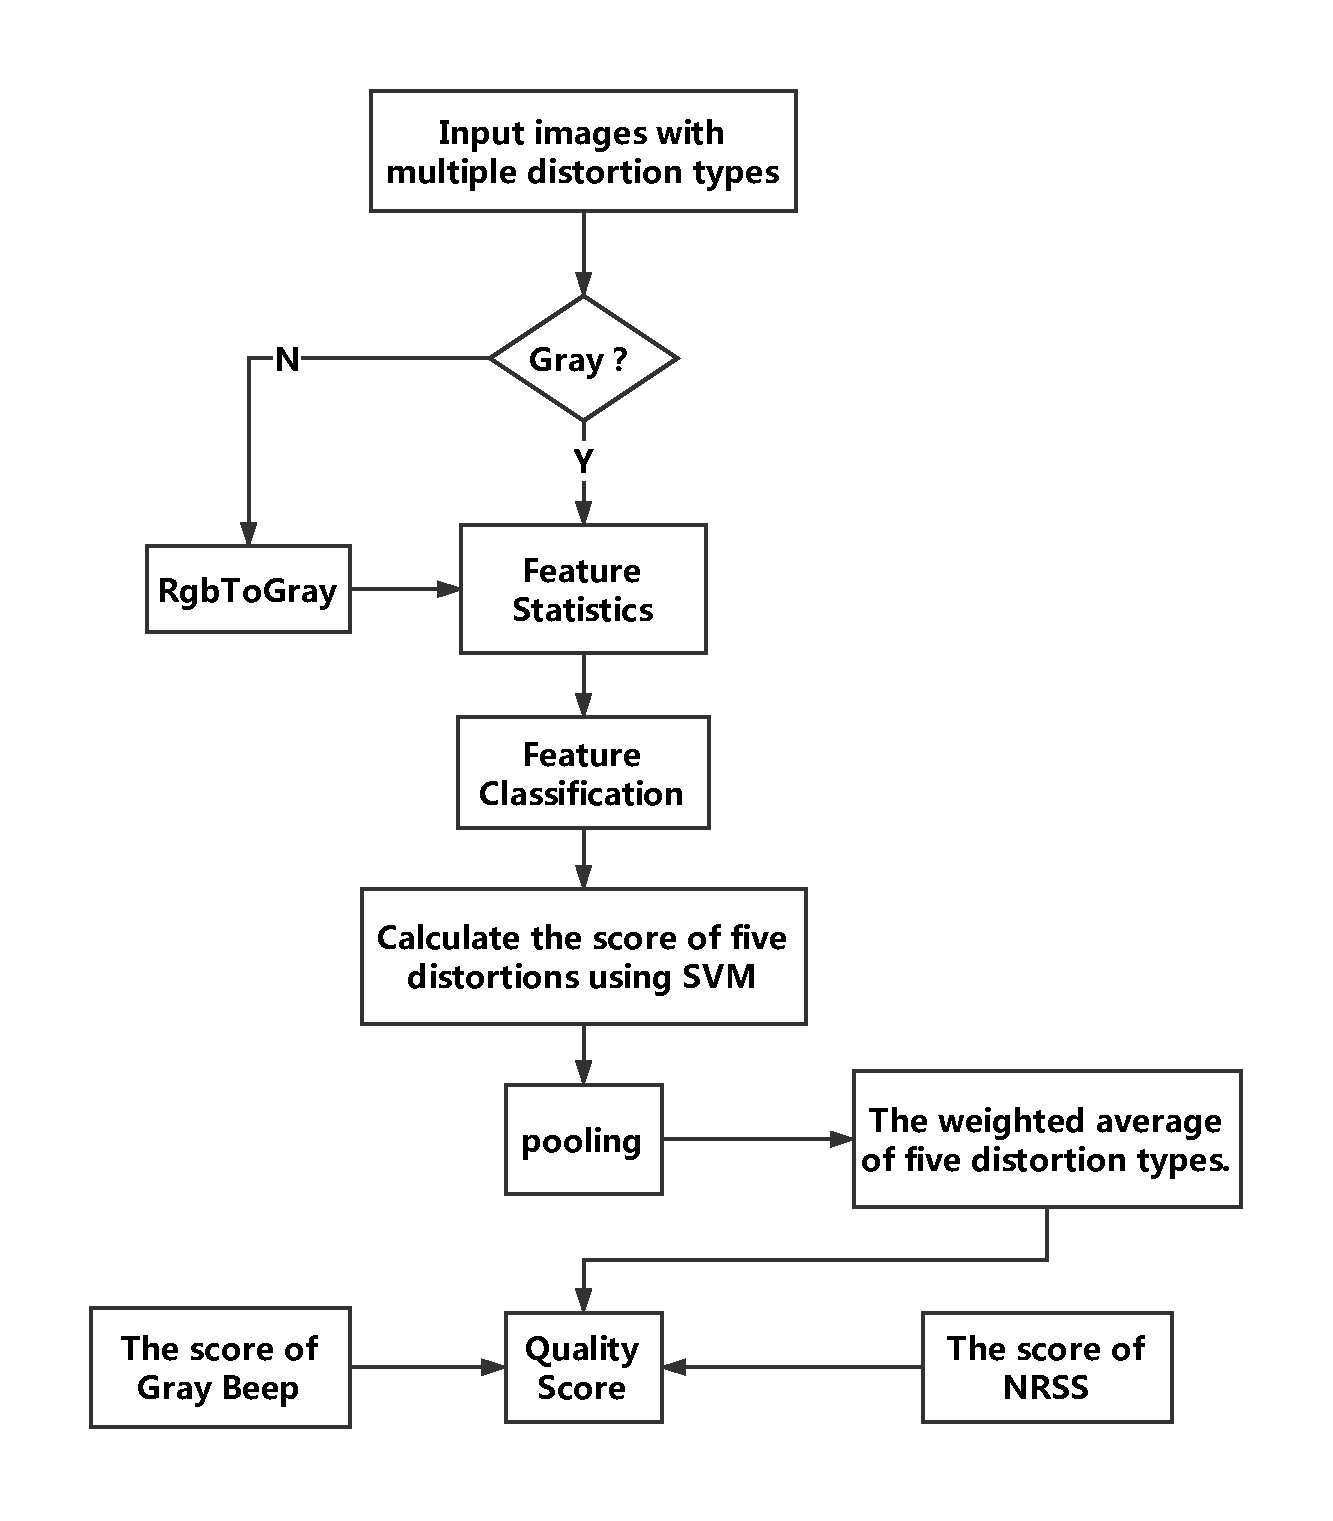
\includegraphics[height=10cm, width=8cm]{images/Main_process.eps}
\caption{Main Process: (1) Judge whether the style of images are gray or not. (2) Extract and classify the features from images. (3) Use SVM to calculate the scores of five distortions respectively. (4) Integrate three steps and get the last results.}
\label{1}
\end{figure}

In this main process, the most vital step is to get the coefficient of each distortion type. This can be divided into some steps. All of first, feature information is got from an image by a wavelet transform over three scales and three orientations using the Daubechies 9/7 wavelet basis. Secondly, using generalized gauss Distribution model is to fit the wavelet coefficients of each subbands. And lastly eighteen-dismentional feature vectors with three directions, three scales and two features are extracted from the final image. In terms of the Generalized Gaussian Distribution mathematical expression, it can be shown as follow:

\begin{equation}
f_{x}\left ( x;\mu ,\sigma ,\gamma \right ) = ae^{-[b|x-\mu|]^{\gamma }}, x\in R
\end{equation}
\begin{equation}
\tau (x) = \int_{0}^{\infty }t^{x-1}e^{-t}dt, x>0
\end{equation}
where $\mu,\sigma^{2}, \gamma$ represent mean, variance and shape-parameter of the distribution. The $x$ is a variable about the different value of the wavelet coefficients of subbands. The coefficient $a$ can be calculated by $a = \beta \gamma /2\tau(1/\gamma)$, and $b = (1/\sigma ) \sqrt{\tau (3/\gamma )\tau (1/\gamma )}$. $\tau (x)$ is a gamma function, which is to build the model of Generalized Gaussian Distribution faster. Besides, in general, the value of the wavelet coefficient is zero-mean since wavelet bases act as band-pass filters. Hence, we just retain two parameters, which are  $\sigma$ and $\gamma$ respectively. The function based on (3) can be formulated as: 

\begin{equation}
f_{x}\left ( x;\sigma ,\gamma \right ) = ae^{-[b|x|]^{\gamma }}, x\in R
\end{equation}

After these above steps, using a training set of distorted images is necessary, and it can classify those images into five different distortion categories, including JPEG, JPEG2000, WN, Blur, and FF. A multiclass SVM with a radial-basis function (RBF) kernel is used to classify a given image into one of the five distortion categories. Lastly, we can get the results through the ratio of these five types of distortion.

As for more specific BIQI's process, firstly, judging the images whether are gray or not  is important for next step after getting the images with multiple distorted types. Then statistics and classification are mainly used to deal with data in order to reduce complexity of computational process. Next step is that calculating the scores in these five distortions, which including Jp2k, JPEG, WN, Blur, FF. Finally, after pooling and tying up these five factors throughout metrics, the quality scores are computed by Eq. (4). 
Overall, this original algorithm can be described by two steps as follows:
(1) SVM is used to classify and calculate the proportion of each distortion type.
(2) Use support vector regression (SVR) and proposed algorithm to obtain the corresponding quality scores from classified distortion type. And next the final results can be computed by weighted mean.
The most proper results ($quality_1$) can be expressed as the following formula:

\begin{equation}
quality_1 = \sum_{i=1}^{5}p_{i}\cdot q_{i}
\end{equation}

In this formula, the $quality_1$ of the image is expressed as a probability-weighted summation. The probability of each distortion in the image is denoted as $p_{i}$, and another parameter represents that the quality scores from each of the five quality assessment algorithms.

%%%%%%%%%%%%%%%%%%%%%%%%%%%%%%%%%%%%%%%%%%


%%%%%%%%%%%%%%%%%%%%%%%%%%%%%%%%%%%%%%%%%%
\subsection{Optimization of NRSS}

There are a large number of NR IQA algorithms recently. However, problems still exist. Although the majority of algorithms can evaluate well images with single distortion type, an amount of images taken by cameras or phones carry usually multiple distortion types and levels. What is more, most of them are hard to be coped with. Consequently, we make an attempt to assess an image with variety distortion types, and improve the quality score as much as possible.

The first improvement is NRSS and it needs to use low-pass filter to handle itself firstly, and many experiments prove that using smoothing filter based on disc model mean filter and gaussian model can create an good reference image for next step. To match the image system better, it is adopted that the $8\times8$ template and the gaussian filter with a variance of 6. Because the human eyes have special reflection on edge information in horizontal and vertical directions, sobel operator is used to extract silhouettes from horizontal and vertical directions respectively. Finding those images with various and abundant gradient information is important, as it can avoid losing some important edge information.

NRSS has great influence on estimating multiple distorted images, especially, those images with blur are extremely obvious. Its general steps can divide into four steps, which include using low-pass filter, getting gradient images by sobel operator, dividing into $8\times8$ blocks and calculating variance, lastly, calculating mean variance. As shown in Figure 2.
%%the image of NRSS
\begin{figure}
\centering
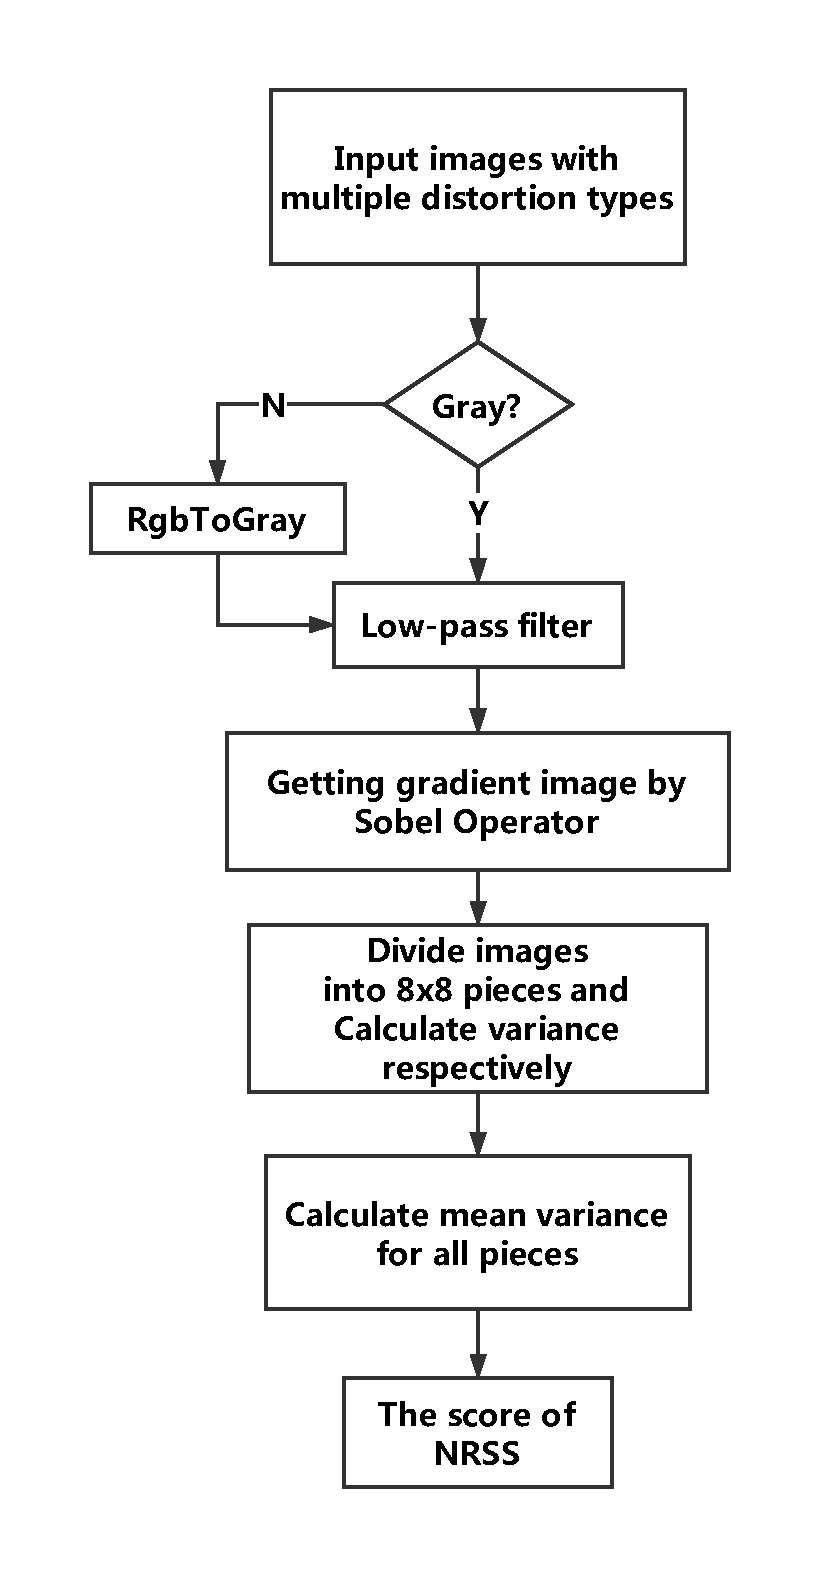
\includegraphics[height=10cm, width=8cm]{images/NRSS.eps}
\caption{NRSS: (1) Judge whether the style of images are gray or not. (2) Use low-pass filter to optimized images. (3) Use Sobel operator to get gradient information. (4) Divide images by fixed module. (5) Calculate mean variance and obtain quality scores.} 
\label{2}
\end{figure}

After calculating the most proper proportion, the $quality_2$ can be expressed as the following formula:

\begin{equation}
quality_2=\frac{quality_1 + nrss}{2}
\end{equation}

In Eq. (5),  $nrss$ is a coefficient and its value is obtained through calculating the mean of gradient. And the $quality_1$ represents original value, which is obtained from BIQI algorithm. Taking the average of the $nrss$ and $quality_1$ is the most proper computing method. 

In general, for this parameter, the results are great on the evaluation of various distortion types, especially blur distortion. It is based on Structural Similarity Index (SSIM) and it is mainly divided into four steps as follow:
(1) The low-pass filter is used to produce reference image. it needs to build a gaussian filter, and after doing lots of experiments in different occasions, the $8\times8$ filter template can achieve the best evaluation results.
(2) It is that extracting gradient information from distortion image and reference image. The major standards that people judge whether the images are clear or not, which are from the edge and contour of images. Hence, using this way to evaluate an image can imitate the attention point of human eyes. 
(3) It is that dividing the gradient image into $8\times8$ blocks and calculating the variance of each blocks. The purpose of dividing into $8\times8$ blocks is to avoid losing some vital edges and the bigger variance of each blocks, the more abundant the gradient information is.
(4)The last step is that calculating SSIM directly. This method that do not need reference images can increase the efficiency in evaluating images, meanwhile, it could decrease the difference with HVS. 

%%%%%%%%%%%%%%%%%%%%%%%%%%%%%%%%%%%%%%%%%%

%%%%%%%%%%%%%%%%%%%%%%%%%%%%%%%%%%%%%%%%%%

\subsection{Optimization of grayscale}
%%grayscale
\par Another added improvement is grayscale, and it also has identical potency like the other distortion’s influence. The extent of grayscale can be described by a threshold. The value can be obtained by counting the numbers of gray series. Meanwhile, calculating the level of grayscale is extremely simple and effective by this statistical number. In most of cases, those proportion over around 50 percents will be regarded as high grayscale. And this figure can be tested on current databases or those distortion images. To increase its accuracy, we add specially the meaning of mean value, because this can be closer to the results. Another apparent point should be noticed is that when a continuous level change in intense, the level of the grayscale is high. 
\par In most real cases, images will contain some certain grayscale, consequently, considering that is another crucial aspect in IQA. In Figure 3, although the process is simple relatively, it still needs to be added to the process of calculating IQA scores. It mainly counts gray series and grayscale, then Eq. (6) is used to compute the proportion of the grayscale.
%%the proportion of Grayscale
\begin{equation}
GHS = \frac{sum}{255} 
\end{equation}

In Eq. (6), the $GHS$ is a ratio indicating the level of the grayscale in an image, and the $sum$ stands for how many grayscales produced.
%%the image of Grayscale
\begin{figure}
\centering
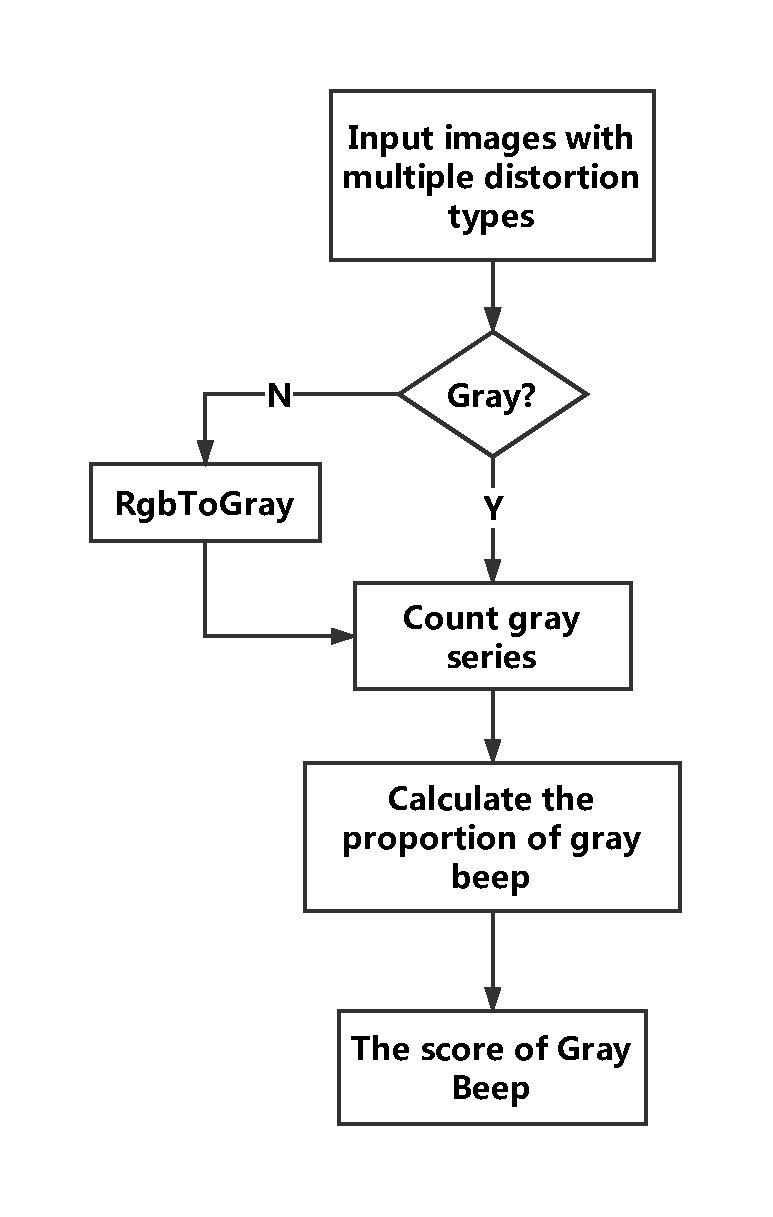
\includegraphics[height=10cm, width=8cm]{images/Gray_Beep.eps}
\caption{Grayscale:  (1) Judge whether the style of images are gray or not.  (2) Compute gray series and its corresponding. (3) Get the scores of grayscale. }
\label{3}
\end{figure}
In Figure 3, judging whether the styles of images are gray or not is important step, and it ensures that next steps could run, and if those images are RGB images, they can deal with this solution through RGBToGray function. Then it needs to count gray series and its corresponding proportion, there is a relatively easy way to compute, it compares whether the difference between the two series is bigger than the critical value, after counting the number of outliers, the proportion of grayscale can be obtained by above Eq. (6). 

%%%%%%%%%%%%%%%%%%%%%%%%%%%%%%%%%%%%%%%%%%

\section{Experiments}
\subsection{Datasets and Settings}

In recent years, plenty of reliable image databases had emerged. For example, Multimedia Information and Communication Technology (MICT), Tampere Image Database (TID2008), Tampere Image Database 2013 (TID2013) and Multiply Distorted Image Database (MDID).

%%MICT
Multimedia Information and Communication Technology  (MICT) database includes 14 reference images and 168 distorted images, and it was created by Toyama University. An image mainly contains two distortion types of JPEG compression and JPEG2000 compression. The MOS value of the database is given by 16 observers, and the value of MOS is [1,5].
%%TID2008
TID2008 database includes 25 reference images and 1700 distorted images. There are 17 kinds of distortion types: additive gaussian noise, additive noise, space position correlation noise, mask noise, mask noise, high frequency noise, impulse noise, quantization noise, gaussian blur, image noise, JPEG compression, JPEG2000 compression, JPEG transmission error, JPEG2000 transmission error, non eccentricity Noise, local distortion, intensity mean shift and contrast change of different intensity.
%%TID2013
TID2013 database is an enhanced version of TID2008 database, including 25 reference images and 3000 distorted images. 
%%MDID
MDID includes 20 reference images and 1600 distorted images. Table 1 presents the detailed information about these IQA databases.



%%Table about database
\begin{table}
% table caption is above the table
\caption{Detailed information of publically available IQA databases.}
\label{tab:1}       % Give a unique label
% For LaTeX tables use
\begin{tabular}{llllll}
\hline\noalign{\smallskip}
Database & MICT & TID2008 & TID2013 & MDID &  \\
\noalign{\smallskip}\hline\noalign{\smallskip}
Database					& 14				& 25					&25					& 20			\\
Number of ref. images		& 196			& 1700				&3000				&1600		\\
Number of dis. images	     	&196				&1700 				&3000  				&1600 		\\
DistortionTypes		    		&2				&17 					&24  					&5 			\\
DistortionLevels	     		&6				&4   					&5   					&4   			\\
RangeScores			   	&1-5				&0-9 				&0-9 				&0-8			\\
Averaged			 		&14.7294			&7.2782  				&7.2126 				&6.4771		\\
ImageFormat			 	&BMP			&BMP  				&BMP 				&BMP		\\
\noalign{\smallskip}\hline
\end{tabular}
\end{table}






%%the reason why choose MDID.
MDID has different characters with other databases. Three views are shown as follow:
(1) Distorted image includes variety distortion types. Meanwhile, the number and levels (from 1 to 4) of distortion for distorted images are random.
(2) Distorted information can be obtained from distorted images.
(3) MDID can be applied into FR and NR image quality assessment problems.
                                                                                                                                                                                                                                                                                                                                                                                                                                                                                                                                                                                                                                                                                                                                                                                                                                                                                                                                                                  
Besides, the reference images from MDID are picked up according to the texture characteristics, varied regions, edges, and details. Making use of these factors, selecting 20 images from different databases are regarded as reference images. Those distorted images from MDID are usually generated by distorting the reference images artificially. In these images, they mainly contain five distortion types, including Gaussian noise (GN), Gaussian blur (GB), contrast change (CC), JPEG. and JPEG2000. Specially, GN is a kind of common distortion type in real image. Meanwhile, GN has many benefits in theoretical derivation or other operation. Another distortion type is Gaussian blur (GB). This is widely used in image acquisition and processing. Besides, JPEG and JPEG 2000 are inevitable factor to decrease image quality scores. In this paper, in order to test and verify the feasibility of proposed algorithm, using natural images with multiple distortion type is necessary, and lastly the consequence need to close to the results of HVS. Overall, caused by various databases, four primary databases will become the important research subjects for our experiments after several times of comparisons.

In Table 1, TID2008 and TID2013 both exceed 15 distortion types. However, it is need to be noticed that each distorted image has only single type of distortion. And the MICT database also has the same character like them. Hence, taking these databases is to compare with MDID, and find whether MDID is great or not. In MDID, arbitrary distortion image includes variety distortion types. This can enclose the real situation. The outcome is that the the proposed algorithm in this paper has positive quality scores \cite{b24}.

For the sake of making a sharp contrast with NR IQA, the classical FR IQA (Peak Signal to Noise Ratio (PSNR)) is used to make a comparison. And the proposed algorithm is tested on the MDID.


\par A algorithm needs to define a criteria to judge whether it is good or not. And it is necessary that an excellent NR or FR algorithm should have a good correlation with HVS. This primary standard is that judging the correlation between subjective scores and objective scores. In this paper, we make use of PLCC, SROCC, KROCC \cite{b25,b26,b27,b28,b29}to judge performance of the algorithm. Pearson product-moment correlation coefficient (PLCC) is easily calculated. It can be shown as:
\begin{equation}
PLCC=\frac{COV(X,Y)}{\delta_{X}\delta_{Y}}
\end{equation}
\par In this Eq. (7), it describes the level of correlation between $X$ and $Y$, the $X$ and $Y$ are regarded as variable, and the $COV(X,Y)$ represents covariance between $X$ and $Y$, and the $\delta_{X}$ and $ \delta_{Y}$ are variance respectively.
The kendall rank-order correlation coefficient (KROCC) and the spearman rank-order correlation coefficient (SROCC) make use of subjective scores and objective scores to estimate their correlation. For KROCC, the $P$ represents the numbers of the same elements between $X$ and $Y$. The $Q$ denotes the logarithm of elements with inconsistencies in $X$ and $Y$. The $X_{0}$ and $Y_{0}$ are the same as mentioned above. For SROCC, $n$ is the size of content. $d$ represents the level of variable \cite{b30,b31,b32}. They can be presented as:
\begin{equation}
KROCC = \frac{P - Q}{\sqrt{(P+Q+X_{0})(P+Q+Y_{0})}}
\end{equation}
\begin{equation}
SROCC = 1 - \frac{6\sum{{d_i}^2}}{n(n^2 - 1)}
\end{equation}

\par It is worth mentioning that we mainly conduct these experiments on macOS Sierra 10.12.6 and Windows. Besides, we use MATLAB to code all of programs. Meanwhile, this experiment is based around a computer, which contains 1.6 GHz Intel Core i5, 8 GB and Intel HD Graphics 6000 1536 MB.


%%%%%%%%%%%%%%%%%%%%%%%%%%%%%%%%%%%%%%%%%%

%%%%%%%%%%%%%%%%%%%%%%%%%%%%%%%%%%%%%%%%%%




\subsection{Optimized parameters}
%% we utilize a probability weighted summation to compute the final BIQI score.
%%Two parameters 

Two improvements are the NRSS and the grayscale respectively, and they as two new factors will be mixed into BIQI. Meanwhile, two parameters will be optimized by comparing the different results calculated by proposed algorithm in this paper. In order to further enhance the positive effects of these two improvements on IQA, we endeavored to compare all kinds of possible significant situations for algorithm's accuracy. And in next experiment, we will test the performance of the proposed algorithm under the condition of blur and noise, because blur and noise are primary influence elements on real images. So, we picked up some reference images and images with multiple distortion types and levels from MDID. And specific information will be shown in Table 2. Four images with different distortion types are displayed in Figure 4-7.  Figure 4 is a reference image, which is prone to compare with others. Figure 5 is an image with noise and Figure 6 is an image with blur, both of them only include a kind of distortion type. The last one is Figure 7, and this image contains the distortions of blur and noise. In these four images, we tested them on the proposed algorithm to illustrate algorithm's performance. From Table 2, the quality score of reference image is largest, while the image with noise and blur is smallest. Obviously, we can find easily that the quality scores are basically equal to our HVS's estimation by observing these four images.

In Table 2, it has a downward trend, along with different distortions. From this table, we can find that blur has the strongest influence on IQA, compared with noise. And in (b), the noise is generated by Gaussian White noise, a matrix of Gaussian white noise with 3 rows and 3 columns is used, and the intensity of output noise is specified in 0.3 in dBW. In (c), the Blur is the Gaussian Blur using a Gaussian low-pass filter, $5\times5$ matrix template and 0.5 standard deviation. Through comparing, we can see that both of them have a great impact on algorithm's performance, it is inevitable that we take more effective actions through mixing NRSS and grayscale into algorithm .


\begin{figure*}
  % include first image
  
\includegraphics[width=0.8\textwidth]{images/image17.eps}
  \caption{Reference}
  \label{fig:sub-first}
  
    % include second image
  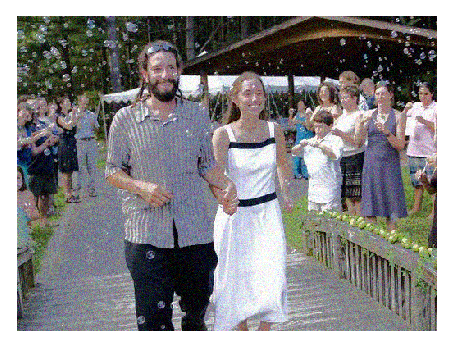
\includegraphics[width=0.8\linewidth]{images/IMAGE1728.eps}  
  \caption{Noise}
  \label{fig:sub-second}
  \end{figure*}
  \begin{figure*}
    % include third image
  
\includegraphics[width=.8\linewidth]{images/IMAGE1704.eps}  
  \caption{Blur}
  \label{fig:sub-third}
  
    % include fourth image
  
\includegraphics[width=.8\linewidth]{images/IMAGE1721.eps}  
  \caption{Noise-Blur}
  \label{fig:sub-fourth}
  
\end{figure*}

%%Table about database
\begin{table}
\caption{The quality scores of an image in different distortion types.}
\label{tab:2}       
\begin{tabular}{llllll}
\hline\noalign{\smallskip}
Types & Reference & Noise & Blur & Noise-Blur &  \\
\noalign{\smallskip}\hline\noalign{\smallskip}
Scores				&67.5681    			&52.8872			&44.2437			&38.8665	\\
\noalign{\smallskip}\hline
\end{tabular}
\end{table}






%%NRSS
\par In order to judge the performance of NRSS and the efficiency in BIQI, there are two experiments to prove this algorithm's reliability. In these experiments, those mentioned criteria are used to judge whether the results are close to HVS or not. And we can validate efficiency through two experiments as follow. 
\par Firstly, we try to change constantly the value of NRSS' probability and find the most proper one in this algorithm. Through manual comparison, we get a set of candidates, and then these possible values are displayed in Table 3. We can find that 0.03 is the most proper result in IQA, and the accuracy of 0.005 has been met the demand of experiment, so finding other coefficient is meaningless. There is description about this digital of 0.03, when the digital for the NRSS is less than 0.03, the NRSS will be mixed into algorithm by using Eq. (5). 


%%Table about NRSS
\begin{table}
\caption{PLCC, SROCC, KROCC under different probability of NRSS.}
\label{tab:3}       
\begin{tabular}{llllllll}
\hline\noalign{\smallskip}
Criteria & 0.025 & 0.03 & 0.035 & 0.04 & 0.05 & 0.06 & \\
\noalign{\smallskip}\hline\noalign{\smallskip}
PLCC	&0.6556    &\textbf{0.6885}	&0.6860 	&0.6626  	&0.6846	&0.6757\\
SROCC	&0.6328    &\textbf{0.6363}	&0.6362 	&0.6349  	&0.6256	&0.6019\\
KROCC	&0.4454    &\textbf{0.4492}	&0.4489 	&0.4478  	&0.4406	&0.4205\\
\noalign{\smallskip}\hline
\end{tabular}
\end{table}




\par Secondly, the compared results between BIQI with NRSS and BIQI with non-NRSS will be displayed, so as to demonstrate that the NRSS is worth existing in this proposed algorithm. Besides, it is apparent that the bigger the probability of NRSS, the more biased the result is. In Table 4, BIQI with NRSS shows better effects than that for non-NRSS. And it represents that NRSS has positive influence on IQA.


%%Table about BIQI and NRSS
\begin{table}
\caption{Comparisons of NRSS and non-NRSS in BIQI.}
\label{tab:4}       
\begin{tabular}{llll}
\hline\noalign{\smallskip}
Type & BIQI with non-NRSS & BIQI with NRSS &\\
\noalign{\smallskip}\hline\noalign{\smallskip}
$PLCC		$  &0.6763    	&0.6885			\\
$SROCC		$  &0.6276     	&0.6363			\\
$KROCC		$  &0.4431    	&0.4492			\\
\noalign{\smallskip}\hline
\end{tabular}
\end{table}







%%Grayscale
\par Another improvement is grayscale, it also plays a vital role in IQA. Similarly, grayscale also requires proof of performance. It is worth noticing that all of the remaining experiments will continue to be done through using the improved algorithm. It means that the proportion of NRSS has been determined, and then it will add another factor of grayscale into BIQI with NRSS. 
\par In general, computing the percentage for grayscale can be divided into two steps, the first step is to statistic and count all gray series, and then it will judge whether gray series happened or not. The second step is that obtaining the probability of grayscale by calculating ratio between the amount of grayscale and total series. Based on above steps, there are plenty of tables to compare and illustrate whether the optimized parameter can show more precise results or not. Besides, some images are presented in Figure 8 and Figure 9.

%%Table about grayscale
\begin{table}
\caption{Proportion of grayscale in multiple distortion image.}
\label{tab:5}       
\begin{tabular}{llllll}
\hline\noalign{\smallskip}
Image & Img0205 & Img0249 & Img0324 & Img0506 &\\
\noalign{\smallskip}\hline\noalign{\smallskip}
Grayscale	  &0.3608    &0.2941	&0.2314 	&0.5569  	\\
\noalign{\smallskip}\hline
\end{tabular}
\end{table}







\begin{figure}[htbp] %  figure placement: here, top, bottom, or page
   \centering
   		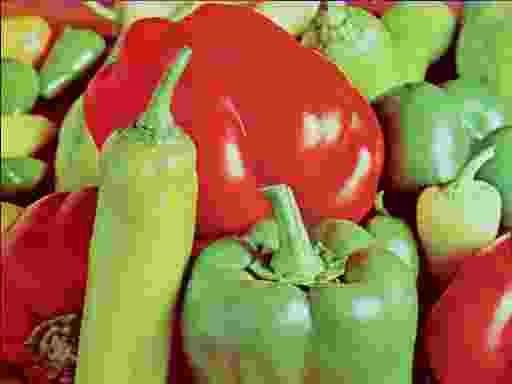
\includegraphics[width=2.3in]{images/img0205.jpg} 
		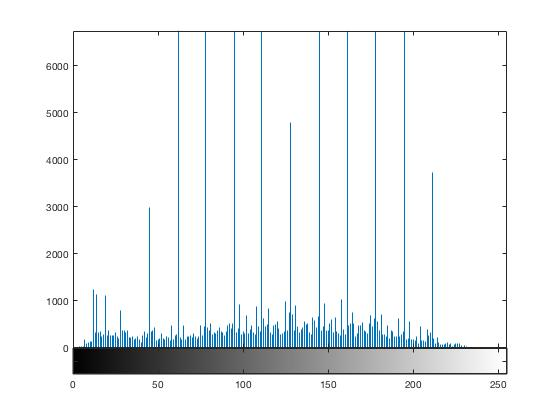
\includegraphics[width=2.3in]{images/imgMDID0205.jpg} 
		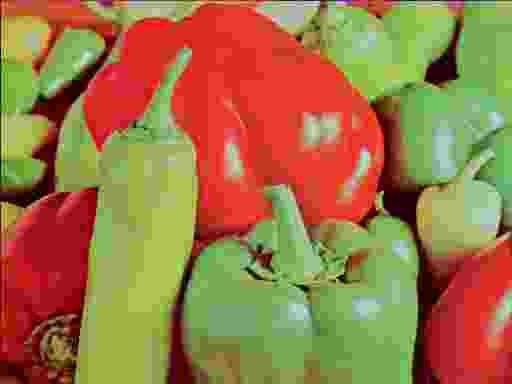
\includegraphics[width=2.3in]{images/img0249.jpg} 
		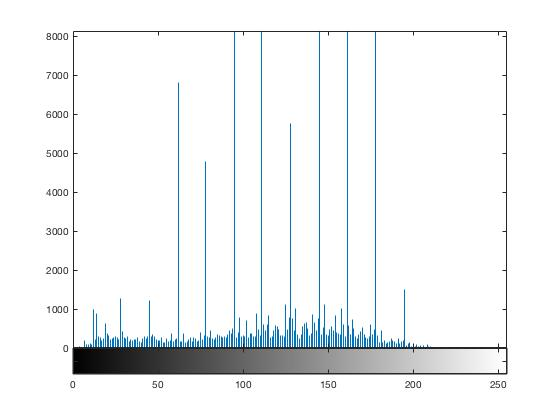
\includegraphics[width=2.3in]{images/imgMDID0249.jpg} 
          	   \caption{The Gray histogram of img0205 and img0249 }
\end{figure}

\begin{figure}[htbp] %  figure placement: here, top, bottom, or page
   \centering
   		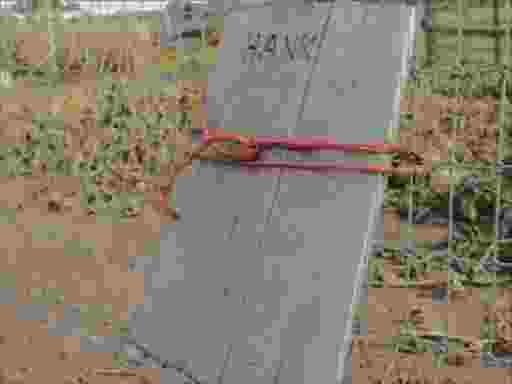
\includegraphics[width=2.3in]{images/img0324.jpg} 
		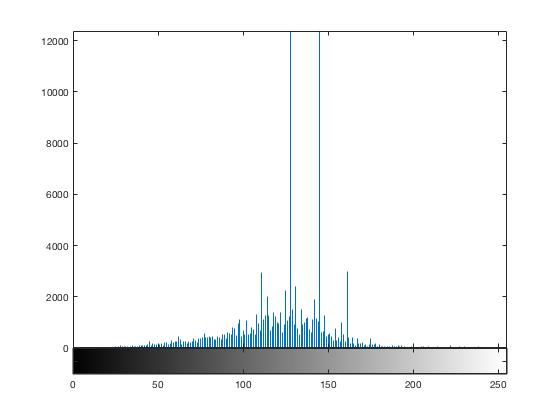
\includegraphics[width=2.3in]{images/imgMDID0324.jpg}    		
   		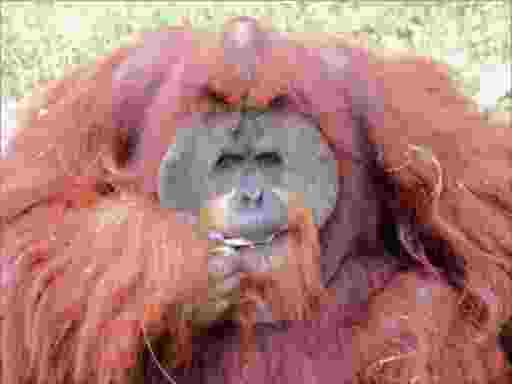
\includegraphics[width=2.3in]{images/img0506.jpg} 
		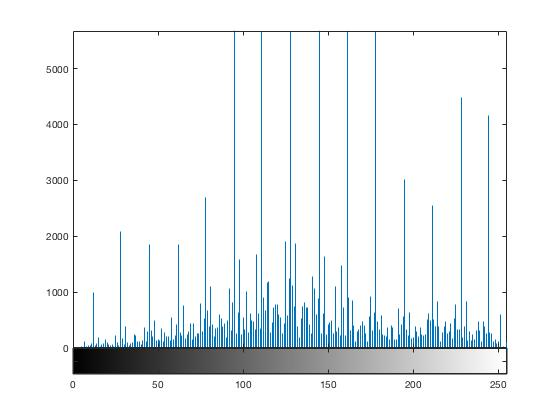
\includegraphics[width=2.3in]{images/imgMDID0506.jpg} 
          	 \caption{The Gray histogram of img0324 and img0506}
\end{figure}

According to above data, grayscale in multiple distortion image has certain influence in IQA, so it is likely to increase the accuracy of algorithm when mixing the grayscale into BIQI. Besides, the results obtained by this way are close to HVS. Some data and images are displayed on Table 5, Figure 8, Figure 9, which are the probability of grayscale and the histograms of gray series in distortion image respectively. The more obvious its change of gray series, the more it represents the serious grayscale. 


%%讲占比
Besides, this improvement will be regarded as a part of quality scores. Consequently, the proportion as a new parameter occupies certain percentage of the last results, and the most appropriate value is around 0.6. 
Table 6 will be shown as follows:  


%%Table about percentage
\begin{table}
\caption{The most appropriate proportion of grayscale in quality scores.}
\label{tab:5}       
\begin{tabular}{lllllll}
\hline\noalign{\smallskip}
Criteria & 0.3 & 0.4 & 0.5 & 0.6 & 0.7 &\\
\noalign{\smallskip}\hline\noalign{\smallskip}
PLCC	&0.6850    	&0.6861		&0.6869 		&\textbf{0.6863}  	&0.6856	\\
SROCC	&0.6347     	&0.6363		&0.6374 		&\textbf{0.6382}  	&0.6263	\\
KROCC	&0.4497    	&0.4513		&0.4524 		&\textbf{0.4530}  	&0.4506	\\
\noalign{\smallskip}\hline
\end{tabular}
\end{table}



%%last result
After getting the proportion of grayscale,
the last results can be expressed as the following formula:
\begin{equation}
 QualityScore=quality_2*(1-GBS*0.60)
\end{equation}



%%Table about percentage
\begin{table}
\caption{PLCC, SROCC, KROCC under different probability of quality scores.}
\label{tab:5}       
\begin{tabular}{lllllll}
\hline\noalign{\smallskip}
Criteria & Database & BIQI & PSNR & Proposed Algorithm &\\
\noalign{\smallskip}\hline\noalign{\smallskip}
$PLCC		$  &MDID    		&0.6763			&0.6610		&\textbf{0.6863}\\
$			$  &TID2008    		&0.5524			&0.5230 		&\textbf{0.5526}\\
$			$  &TID2013    		&0.5323			&0.5533 		&\textbf{0.5744}\\
$			$  &MICT    		&0.5232			&0.5433 		&\textbf{0.5524}\\ %%MICT
$SROCC		$  &MDID    		&0.6276			&0.6382 		&\textbf{0.6390}\\
$			$  &TID2008    		&0.5467			&0.5264 		&\textbf{0.5530}\\
$			$  &TID2013    		&0.5326			&0.5235 		&\textbf{0.5684}\\
$			$  &MICT    		&0.5132			&0.5343 		&\textbf{0.5456}\\ %%MICT
$KROCC		$  &MDID    		&0.4431			&0.4530 		&\textbf{0.4730}\\
$			$  &TID2008    		&0.3836			&0.3695 		&\textbf{0.4020}\\
$			$  &TID2013    		&0.4222			&0.4243 		&\textbf{0.4424}\\
$			$  &MICT    		&0.4012			&0.4222 		&\textbf{0.4314}\\ %%MICT
\noalign{\smallskip}\hline
\end{tabular}
\end{table}





%%different databases
Ultimately, the algorithm is tested on other databases like MDID, TID2008, TID2013 and MICT. The results obtained from different databases show that this algorithm is more efficient than consequences of other algorithms. From Table 7, we can find: (1) PSNR performs the worst, because the values for LCC, SROCC and KROCC are the smallest while that of the proposed algorithm are the largest; (2) Followed by PNSR, it is BIQI, which presents better results than PNSR; (3) In those databases with multiple distortion types and levels, there is a significant progress, compared with other algorithms. To further confirm their values, we adopt computational time to describe the practicability and effectiveness of the proposed algorithm. 
\par To estimate the computational time of different picture with one or more distorted types conveniently, we show the computational time of the algorithm under different distorted types of pictures in Table 8.


%%Table about computational time 
\begin{table}
\caption{computational time.}
\label{tab:5}       
\begin{tabular}{lllllll}
\hline\noalign{\smallskip}
Image & Img with Blur & Img with noise & Img with blur and noise & Average &\\
\noalign{\smallskip}\hline\noalign{\smallskip}
Grayscale	&2.3277    &2.1944	&2.1107   	&2.1963		\\
\noalign{\smallskip}\hline
\end{tabular}
\end{table}


Analogously, Table 8 as typical examples are used to test the speed of the proposed algorithm. Meanwhile, we compute the averaged computational time on all of images from MDID to show more general situation.
%%%%%%%%%%%%%%%%%%%%%%%%%%%%%%%%%%%%%%%%%%
\section{Conclusion}

In this letter, we proposed a new approach with NRSS and grayscale, and it stems from BIQI. This algorithm not only gets the positive quality score, but also encloses the judgement of HVS. After mixing NRSS and grayscale into BIQI, it can recognize more accurately images with multiple distortion types. In conclusion, although the proposed algorithm should be noticed that the runtime of training model should be improved, the overall better performance may be obtained as the proposed NR algorithm that correlates better with human perception. 
%%%%%%%%%%%%%%%%%%%%%%%%%%%%%%%%%%%%%%%%%%



%\section*{Acknowledgement}

%%%%%%%%%%%%%%%%%%%%%%%%%%%%%%%%%%%%%%%%%%
%%\acknowledgments{This research was funded by the National Natural Science Foundation of China (61622205, 61872436), the Fujian Provincial Natural Science Foundation of China (2018J01573, 2018J01571), the Fujian Provincial High School Natural Science Foundation of China (JZ160472), Fujian Province Universities and Colleges (JK2015033), the project of New Century Excellent Talents in College of Fujian and distinguished young researchers in College of Fujian.}


\begin{acknowledgements}
This research was funded by the National Natural Science Foundation of China (61622205, 61872436), the Fujian Provincial Natural Science Foundation of China (2018J01573, 2018J01571), the Fujian Provincial High School Natural Science Foundation of China (JZ160472), the project of New Century Excellent Talents in College of Fujian and distinguished young researchers in College of Fujian.
\end{acknowledgements}

%%%%%%%%%%%%%%%%%%%%%%%%%%%%%%%%%%%%%%%%%%

%%%%%%%%%%%%%%%%%%%%%%%%%%%%%%%%%%%%%%%%%%
\vspace{6pt} 

%%%%%%%%%%%%%%%%%%%%%%%%%%%%%%%%%%%%%%%%%%
%% optional
%\supplementary{The following are available online at \linksupplementary{s1}, Figure S1: title, Table S1: title, Video S1: title.}

% Only for the journal Methods and Protocols:
% If you wish to submit a video article, please do so with any other supplementary material.
% \supplementary{The following are available at \linksupplementary{s1}, Figure S1: title, Table S1: title, Video S1: title. A supporting video article is available at doi: link.}








% Non-BibTeX users please use
\begin{thebibliography}{99}
%
% and use \bibitem to create references. Consult the Instructions
% for authors for reference list style.
%
\bibitem{b1} Z. Wang, H. R. Sheikh, and A. C. Bovik, “No-reference perceptual quality assessment of JPEG compressed images," in Proc. IEEE ICIP, 2002, vol. 1, pp. 477–480.
\bibitem{b2} H. R. Sheikh, A. C. Bovik, and L. K. Cormack, “No-reference quality assessment using natural scene statistics: JPEG2000,” IEEE Trans. Image Processing, vol. 14, no. 11, pp. 1918–1927, 2005.
\bibitem{b3} P. Marziliano, F. Dufaux, S. Winkler, and T. Ebrahimi, “Perceptual blur and ringing metrics: Application to JPEG2000," Signal Processing:Image Communication, vol. 19, no. 2, pp. 163–172, 2004.
\bibitem{b4}A.K. Moorthy, A.C. Bovik, A two-step framework for constructing blind image quality indices, IEEE Signal Process. Lett. 17 (2010) 513–516.
\bibitem{b5}N. Ponomarenko, V. Lukin, A. Zelensky, K. Egiazarian, M. Carli, F. Battisti, TID2008 – a database for evaluation of full-reference visual quality assessment metrics, in: Adv. Modern Radioelectron, 10 (2009) 30–45.
\bibitem{b6} H. R. Sheikh, M. F. Sabir, and A. C. Bovik, “A statistical evaluation of recent full reference image quality assessment algorithms,” IEEE Trans. Image Processing, vol. 15, no. 11, pp. 3440–3451, Nov. 2006.
\bibitem{b7} Sun, Wen, F. Zhou, and Q. Liao. "MDID: A multiply distorted image database for image quality assessment." Pattern Recognition 61(2017):153-168.
\bibitem{b8}WANG Zhou, BOVIK A C. Modern image quality assessment [M]. New York: Morgan and Clay pool Publishing Company, 2006:20-30.
\bibitem{b9}WANG Zhou, BOVIK A C, SHEIKH H R, er al. Image quality assessment: from error visibility to structural similarity [J]. IEEE Trans on Image Processing, 2004, 13(4): 600-612.
\bibitem{b10} Tong H,Li M, Zhang H J,et al. No-reference quality assessment for JPEG2000 compressed images[C]//Proceedings of International Conference on Image Processing,2004, 5:3539-3542.
\bibitem{b11} Sazzad Z M P,Kawayoke Y,Horita Y.No reference image quality assessment for JPEG2000 based on spatial features[J]. Signal Processing:Image Communication,2008, 23(4):257-268.
\bibitem{b12} Sheikh H R,Bovik A C,Cormack L.No-reference quality assessment using natural scene statistics:JPEG2000[J]. IEEE Trans on Image Processing,2005,14(11): 1918-1927.
\bibitem{b13} Caviedes J, Oberti F.A new sharpness metric based on local kurtosis, edge and energy information[J]. Signal Processing Image Communication, 2004, 19(2):147-161. 
\bibitem{b14} Ferzli R, Karam L J.A no-reference objective image sharpness metric based on the notion of Just Notice- able Blur(JNB)[J].IEEE Trans on Image Processing,2009,18(4):717-728. 
\bibitem{b15} ZhuX, PeymanM. A no-reference sharpness metric sensitive to blur and noise[J].Quality of Multimedia Experience,2009(1):64-69.
\bibitem{b16} Saad M A, Bovik A C, Charrier C.A DCT statistics based blind image quality index[J].Signal Processing Letters, 2010,17(6):583-586.
\bibitem{b17} Saad M A, Bovik A C, Charrier C.DCT statistics model based blind image quality assessment[C]//Proceedings of the 18th IEEE International Conference on Image Processing(ICIP),2011:3093-3096.
\bibitem{b18}Mittal A, Moorthy A K, Bovik A C.No-reference image quality assessment in the spatial domain[J].IEEE Trans on Image Processing,2012,21(12):4695-4708.
\bibitem{b19} Ruderman D L.The statistics of natural images[J].Network: Computation in Neural Systems,1994,5(4):517-548.
\bibitem{b20} Mittal A,Soundararajan R, Bovik A C. Making a “completely blind” image quality analyzer[J].Signal Processing Letters,2013,20(3):209-212.
\bibitem{b21} Li C F, Bovik A C,Wu X J.Blind image quality assessment using a general regression neural network[J].IEEE Trans on Neural Networks,2011,22(5):793-799.

\bibitem{b22} Edwin H Land. The retinex theory of color vision [J]. Scientific American, 1977, 237(6): 108-129.
\bibitem{b23} Jayant N.Signal compression: technology targets and research directions [J]. IEEE Journal on SelectedAreas in Communication, 1922, 10(5):796-818.
\bibitem{b24} Wang Z, Bovik A C, SheikhH R, et al. Image quality assessment: from error measurement to structural similarity [J]. IEEE Trans on ImageProcessing, 2004, 13(1): 1-14.
\bibitem{b25}Lehmann, E. L.; Casella, George (1998). Theory of Point Estimation (2nd ed.). New York: Springer. ISBN 0-387-98502-6. MR 1639875.
\bibitem{b26}Wackerly, Dennis; Mendenhall, William; Scheaffer, Richard L. (2008). Mathematical Statistics with Applications (7 ed.). Belmont, CA, USA: Thomson Higher Education. ISBN 0-495-38508-5.
\bibitem{b27}Steel, R.G.D, and Torrie, J. H., Principles and Procedures of Statistics with Special Reference to the Biological Sciences., McGraw Hill, 1960, page 288.
\bibitem{b28}Mood, A.; Graybill, F.; Boes, D. (1974). Introduction to the Theory of Statistics (3rd ed.). McGraw-Hill. p. 229.
\bibitem{b29}DeGroot, Morris H. (1980). Probability and Statistics (2nd ed.). Addison-Wesley.
\bibitem{b30}Jun Yu, Chaoqun Hong, Yong Rui, Dacheng Tao, Multitask Autoencoder Model for Recovering Human Poses, IEEE Transactions on Industrial Electronics, vol. 65, no. 6, pp. 5060-5068, 2018.
\bibitem{b31}Jun Yu, Xiaokang Yang, Fei Gao, Dacheng Tao, Deep Multimodal Distance Metric Learning Using Click Constraints for Image Ranking, IEEE Transactions on Cybernetics, vol. 47, no. 12, pp. 4014 – 4024, 2017.
\bibitem{b32}Jun Yu, Dacheng Tao, Yong Rui, Meng Wang, Learning to Rank using User Clicks and Visual Features for Image Retrieval, IEEE Transactions on Cybernetics, vol. 45, no. 4, pp. 767-779, 2015.
\bibitem{b33}WeipengWu, ChaoqunHong, YongXie, LiangChen. (2018). Image Quality Assessment Based on BIQI with Gray Beep.4632-4639. 10.1109/BigData.2018.8622098. 
\bibitem{b34}The [https://github.com/David19970306/Blind-Image-quality-assessment] data used to support the findings of this study are included within the article.



\end{thebibliography}

\end{document}
% end of file template.tex

